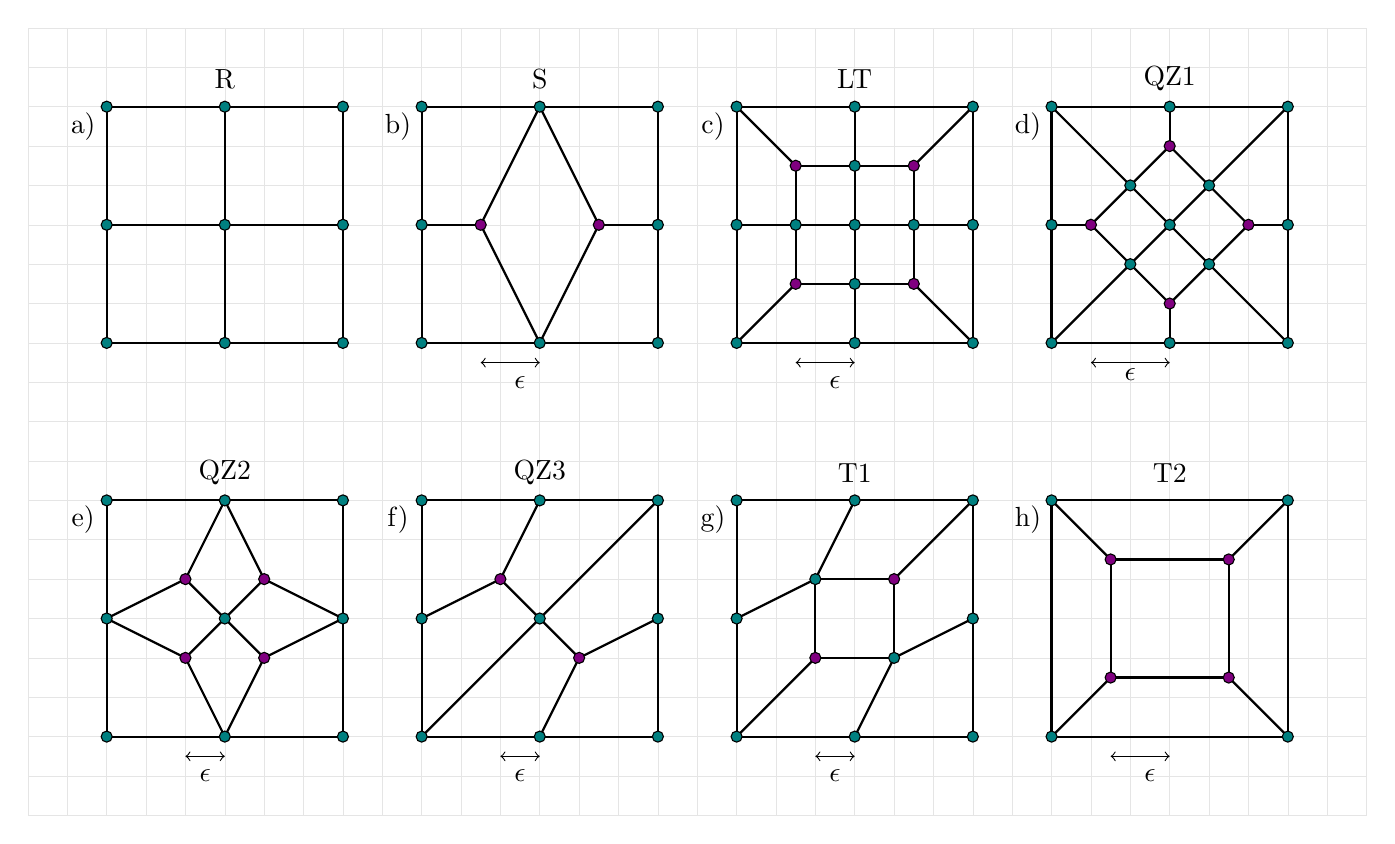
\begin{tikzpicture}
%\draw[fill=gray!23,gray!23](0,0) rectangle (5,5);
\draw[step=0.5cm,gray!20,very thin] (0,0) grid (17,10); %background grid

%%%%%%%%%%%%%%%%%%%%%%%%%%%%%%%%%%%%%%%%%%%%%%%%%%%%%%%%%%
\node[] at (0.7,3.75) {e)};
\draw[thick] (1,1) -- (4,1) -- (4,4) -- (1,4) -- cycle;  

\draw[thick] (1,2.5)--(2,3)--(2.5,4)--(3,3)--(4,2.5)--(3,2)--(2.5,1)--(2,2)--cycle;
\draw[thick] (2,2)--(3,3);
\draw[thick] (2,3)--(3,2);

\draw[black,fill=teal] (1,1)   circle (2pt);
\draw[black,fill=teal] (1,4)   circle (2pt);
\draw[black,fill=teal] (4,1)   circle (2pt);
\draw[black,fill=teal] (4,4)   circle (2pt);
\draw[black,fill=teal] (2.5,2.5)   circle (2pt);

\draw[black,fill=teal] (1,2.5)   circle (2pt);
\draw[black,fill=teal] (4,2.5)   circle (2pt);
\draw[black,fill=teal] (2.5,1)   circle (2pt);
\draw[black,fill=teal] (2.5,4)   circle (2pt);

\draw[black,fill=violet] (2,2)   circle (2pt);
\draw[black,fill=violet] (3,2)   circle (2pt);
\draw[black,fill=violet] (2,3)   circle (2pt);
\draw[black,fill=violet] (3,3)   circle (2pt);

\draw[<->] (2,0.75)--(2.5,0.75); \node[] at (2.25,0.5) {$\epsilon$};

\node[] at (2.5,4.35) {QZ2};

%%%%%%%%%%%%%%%%%%%%%%%%%%%%%%%%%%%%%%%%%%%%%%%%%%%%%%%%%%%%%
\node[] at (4.7,3.75) {f)};
\draw[thick] (5,1) -- (8,1) -- (8,4) -- (5,4) -- cycle;  


\draw[thick] (6.5,1)--(7,2)--(8,2.5) ; 
\draw[thick] (5,2.5)--(6,3)--(6.5,4) ; 
\draw[thick] (6,3)--(7,2);
\draw[thick] (5,1)--(8,4);

\draw[black,fill=teal] (5,1)   circle (2pt);
\draw[black,fill=teal] (5,4)   circle (2pt);
\draw[black,fill=teal] (8,1)   circle (2pt);
\draw[black,fill=teal] (8,4)   circle (2pt);
\draw[black,fill=teal] (6.5,2.5)  circle (2pt);
\draw[black,fill=teal] (5,2.5)   circle (2pt);
\draw[black,fill=teal] (8,2.5)   circle (2pt);
\draw[black,fill=teal] (6.5,1)   circle (2pt);
\draw[black,fill=teal] (6.5,4)   circle (2pt);

\draw[black,fill=violet] (6,3)   circle (2pt);
\draw[black,fill=violet] (7,2)   circle (2pt);


\draw[<->] (6,0.75)--(6.5,0.75); \node[] at (6.25,0.5) {$\epsilon$};

\node[] at (6.5,4.35) {QZ3};

%%%%%%%%%%%%%%%%%%%%%%%%%%%%%%%%%%%%%%%%%%%%%%%%%%%%%%%%%%%%%
\node[] at (8.7,3.75) {g)};
\draw[thick] (9,1) -- (12,1) -- (12,4) -- (9,4) -- cycle;  
\draw[thick] (10,2)--(11,2)--(11,3)--(10,3)--cycle; 
\draw[thick] (9,1)--(10,2);
\draw[thick] (11,3)--(12,4);
\draw[thick] (10.5,1)--(11,2)--(12,2.5);
\draw[thick] (9,2.5)--(10,3)--(10.5,4);

\draw[black,fill=teal] (9,1)   circle (2pt);
\draw[black,fill=teal] (10.5,1)   circle (2pt);
\draw[black,fill=teal] (12,1)   circle (2pt);
\draw[black,fill=teal] (9,2.5)   circle (2pt);
\draw[black,fill=teal] (12,2.5)   circle (2pt);
\draw[black,fill=teal] (9,4)   circle (2pt);
\draw[black,fill=teal] (10.5,4)   circle (2pt);
\draw[black,fill=teal] (12,4)   circle (2pt);
\draw[black,fill=teal] (10,3)   circle (2pt);
\draw[black,fill=teal] (11,2)   circle (2pt);

\draw[black,fill=violet] (10,2)   circle (2pt);
\draw[black,fill=violet] (11,3)   circle (2pt);


\draw[<->] (10,0.75)--(10.5,0.75); \node[] at (10.25,0.5) {$\epsilon$};

\node[] at (10.5,4.35) {T1};


%%%%%%%%%%%%%%%%%%%%%%%%%%%%%%%%%%%%%%%%%%%%%%%%%%%%%%%%%%%
\node[] at (12.7,3.75) {h)};
\draw[thick] (13,1) -- (16,1) -- (16,4) -- (13,4) -- cycle;  


\draw[thick] (13.75,1.75)--(15.25,1.75)--(15.25,3.25)--(13.75,3.25)--cycle; 
\draw[thick] (13,1)--(13.75,1.75); 
\draw[thick] (16,1)--(15.25,1.75); 
\draw[thick] (13,4)--(13.75,3.25); 
\draw[thick] (16,4)--(15.25,3.25); 

\draw[black,fill=teal] (13,1)   circle (2pt);
\draw[black,fill=teal] (16,1)   circle (2pt);
\draw[black,fill=teal] (13,4)   circle (2pt);
\draw[black,fill=teal] (16,4)   circle (2pt);

\draw[black,fill=violet] (13.75,1.75)   circle (2pt);
\draw[black,fill=violet] (13.75,3.25)   circle (2pt);
\draw[black,fill=violet] (15.25,1.75)   circle (2pt);
\draw[black,fill=violet] (15.25,3.25)   circle (2pt);

\draw[<->] (13.75,0.75)--(14.5,0.75); \node[] at (14.25,0.5) {$\epsilon$};

\node[] at (14.5,4.35) {T2};

%%%%%%%%%%%%%%%%%%%%%%%%%%%%%%%%%%%%%%%%%%%%%%%%%%%%%%%%%%%
%R 
%%%%%%%%%%%%%%%%%%%%%%%%%%%%%%%
\node[] at (0.7,8.75) {a)};
\draw[thick] (1,6) -- (4,6) -- (4,9) -- (1,9) -- cycle;  

\draw[thick] (2.5,6) -- (2.5,9) -- cycle;  
\draw[thick] (1,7.5) -- (4,7.5) -- cycle;  

\draw[black,fill=teal] (1,6)   circle (2pt);
\draw[black,fill=teal] (2.5,6)   circle (2pt);
\draw[black,fill=teal] (4,6)   circle (2pt);

\draw[black,fill=teal] (1,7.5)   circle (2pt);
\draw[black,fill=teal] (2.5,7.5)   circle (2pt);
\draw[black,fill=teal] (4,7.5)   circle (2pt);

\draw[black,fill=teal] (1,9)   circle (2pt);
\draw[black,fill=teal] (2.5,9)   circle (2pt);
\draw[black,fill=teal] (4,9)   circle (2pt);

%\draw[<->] (1,5.75)--(4,5.75);
%\node[] at (2.5,5.5) {$h$};


\node[] at (2.5,9.35) {R};


%%%%%%%%%%%%%%%%%%%%%%%%%%%%%%%%%%%%%%%%%%%%%%%%%%%%%%%%%%%
\node[] at (4.7,8.75) {b)};
\draw[thick] (5,6) -- (8,6) -- (8,9) -- (5,9) -- cycle;  
\draw[thick] (6.5,6)--(7.25,7.5)--(6.5,9)--(5.75,7.5) -- cycle;  
\draw[thick] (5,7.5) -- (5.75,7.5);  
\draw[thick] (7.25,7.5) -- (8,7.5);  
\draw[black,fill=teal] (5,6) circle (2pt);
\draw[black,fill=teal] (6.5,6) circle (2pt);
\draw[black,fill=teal] (8,6) circle (2pt);
\draw[black,fill=teal] (5,7.5) circle (2pt);
\draw[black,fill=violet] (5.75,7.5) circle (2pt);
\draw[black,fill=violet] (7.25,7.5) circle (2pt);
\draw[black,fill=teal] (8,7.5) circle (2pt);
\draw[black,fill=teal] (5,9) circle (2pt);
\draw[black,fill=teal] (6.5,9) circle (2pt);
\draw[black,fill=teal] (8,9) circle (2pt);

\draw[<->] (5.75,5.75)--(6.5,5.75); \node[] at (6.25,5.5) {$\epsilon$};

\node[] at (6.5,9.35) {S};

%%%%%%%%%%%%%%%%%%%%%%%%%%%%%%%%%%%%%%%%%%%%%%%%%%%%%%%%%%%%%
\node[] at (8.7,8.75) {c)};
\draw[thick] (9,6) -- (12,6) -- (12,9) -- (9,9) -- cycle;  
\draw[thick] (9.75,6.75)--(11.25,6.75)--(11.25,8.25)--(9.75,8.25) -- cycle;  

\draw[thick] (9,6) -- (9.75,6.75);  
\draw[thick] (11.25,8.25) -- (12,9);  
\draw[thick] (9,9) -- (9.75,8.25);  
\draw[thick] (11.25,6.75) -- (12,6);  
\draw[thick] (9,7.5) -- (12,7.5);  
\draw[thick] (10.5,6) -- (10.5,9);  

\draw[black,fill=teal] (9,6)  circle (2pt);
\draw[black,fill=teal] (10.5,6)  circle (2pt);
\draw[black,fill=teal] (12,6)   circle (2pt);
\draw[black,fill=teal] (9,7.5)  circle (2pt);
\draw[black,fill=teal] (10.5,7.5)  circle (2pt);
\draw[black,fill=teal] (12,7.5)   circle (2pt);
\draw[black,fill=teal] (9,9)  circle (2pt);
\draw[black,fill=teal] (10.5,9)  circle (2pt);
\draw[black,fill=teal] (12,9)   circle (2pt);

\draw[black,fill=teal] (10.5,8.25)   circle (2pt);
\draw[black,fill=teal] (10.5,6.75)   circle (2pt);
\draw[black,fill=teal] (9.75,7.5)   circle (2pt);
\draw[black,fill=teal] (11.25,7.5)   circle (2pt);

\draw[black,fill=violet] (9.75,6.75)  circle (2pt);
\draw[black,fill=violet] (11.25,6.75)  circle (2pt);
\draw[black,fill=violet] (9.75,8.25)  circle (2pt);
\draw[black,fill=violet] (11.25,8.25)  circle (2pt);


\draw[<->] (9.75,5.75)--(10.5,5.75); \node[] at (10.25,5.5) {$\epsilon$};

\node[] at (10.5,9.35) {LT};

%%%%%%%%%%%%%%%%%%%%%%%%%%%%%%%%%%%%%%%%%%%%%%%%%%%%%%%%%%%
\node[] at (12.7,8.75) {d)};
\draw[thick] (13,6) -- (16,6) -- (16,9) -- (13,9) -- cycle;  

\draw[thick] (13,6) -- (16,9) ;
\draw[thick] (13,9) -- (16,6) ;

\draw[thick] (13.5,7.5)--(14.5,6.5)--(15.5,7.5)--(14.5,8.5) -- cycle;
\draw[thick] (13,7.5) -- (13.5,7.5) ;
\draw[thick] (15.5,7.5) -- (16,7.5) ;
\draw[thick] (14.5,6) -- (14.5,6.5) ;
\draw[thick] (14.5,8.5) -- (14.5,9) ;

\draw[black,fill=teal] (13,6)   circle (2pt);
\draw[black,fill=teal] (14.5,6)   circle (2pt);
\draw[black,fill=teal] (16,6)   circle (2pt);
\draw[black,fill=teal] (13,7.5)   circle (2pt);
\draw[black,fill=teal] (14.5,7.5)   circle (2pt);
\draw[black,fill=teal] (16,7.5)   circle (2pt);
\draw[black,fill=teal] (13,9)   circle (2pt);
\draw[black,fill=teal] (14.5,9)   circle (2pt);
\draw[black,fill=teal] (16,9)   circle (2pt);

\draw[black,fill=teal] (14,7)   circle (2pt);
\draw[black,fill=teal] (15,7)   circle (2pt);
\draw[black,fill=teal] (14,8)   circle (2pt);
\draw[black,fill=teal] (15,8)   circle (2pt);

\draw[black,fill=violet] (14.5,6.5)   circle (2pt);
\draw[black,fill=violet] (14.5,8.5)   circle (2pt);
\draw[black,fill=violet] (13.5,7.5)   circle (2pt);
\draw[black,fill=violet] (15.5,7.5)   circle (2pt);

\draw[<->] (13.5,5.75)--(14.5,5.75); \node[] at (14,5.6) {$\epsilon$};

\node[] at (14.5,9.35) {QZ1};

\end{tikzpicture}
